\documentclass{article}
\usepackage{graphicx}
\usepackage{listings} % nice code layout
\usepackage[section]{placeins}
\usepackage{xcolor}
\usepackage[utf8]{inputenc}
\lstset{language = Verilog}
\graphicspath{ {./images/} }

\author{Justin Bui}
\title{Reaction Timer FPGA Implementation}

\begin{document}

\maketitle
\newpage

\tableofcontents
\newpage

\section{Introduction}
This document outlines the Reaction Timer project designed for ELC 5396. This project makes use of the Digilent NEXYS 4 Artix-7 FPGA development board to implement a reaction timer, which measures the response to a randomly generated stimulus. The document below includes the ASMD diagram, functional discription, and thought process behind my programming decissions, as well as testing and performance verification notes. 

\section{Project Requirements}
The Reaction Timer requirements are outlined in problem number 6.5.6 of FPGA Prototyping By SystemVerilog Examples, by Pong Chu. The project is designed to measure the reaction time to a visual stimulus. The design uses the following criteria:

\begin{enumerate}
	\item Three Input Buttons: Clear, Start, and Stop
	\item Pressing the Clear button returns the program to the initial state.
	\item Pressing the Start button initializes the test.
	\item After a random time between 2 and 15 seconds, the stimulus LED is turned on and the reaction timer is started.
	\item The player then has up to one second to press the Stop button. If the timer reaches one second, the player "loses".
	\item Pressing the Stop button before the stimulus is generated results in a "false start", producing an error
\end{enumerate} 

In addition to the 7-Segment display, I have implemented one of the RGB LEDs to allow for state identification. This not only allows for a more visable game interface, but allows for debugging if necessary. The 7-Segment display will show different values, depending on the state of the game. The following table identifies the 7-Segment Display and RGB LED values for the particular states.

\begin{table}[h!]
	\begin{center}
		\caption{State Vales of 7-Segment Display and RGB LED}
		\label{table:table1}
		\begin{tabular}{l l l}
			\textbf{State} & \textbf{7-Segment Display} & \textbf{RGB LED}\\
			\hline
			Ready & H I 0 0 & Blue\\
			Start & 0 0 0 0 & Blue\\
			Game & Run Time & Off\\
			Error & 9 9 9 9 & Yellow\\
			Win & Reflex Time & Green\\
			Lose & 1 0 0 0 & Red
		\end{tabular}
	\end{center}
\end{table}
\newpage

\section{Thought Process and ASMD}
At a high level, the reaction timer can be broken down in to a few core functions, those being the timing element(s) and the display element(s). The textbook provides great code examples for both of these elements, and I have implemented my own version of each for this design. In addition to the timing and display elements, a state machine can be used to better control the programs flow and operation. As you can see from the table on page 3, I have designed this system to make use of 6 states (Ready, Start, Game, Error, Win and Lose). A brief descrption of each state can be found below.

\medskip
\textbf{Ready:}The Ready state is used as my default state, in which the game is held until the player presses the Start button (BTNR). If the player presses the Clear button (BTNC) at any time, the system returns to the Ready state.

\smallskip
\textbf{Start:}When the Start button is pressed, a random number is generated and the timer begins to count towards that random number. When the random number of seconds has been reached, the device moves to the Game state. If the user presses the stop buttong when in this state, the system registers a "false start", and the system moves in to the Error state.

\smallskip
\textbf{Game: }When the Stimulus LED (LED0) is first turned on, the player has up to 1 second to press the Stop button (BTNL). If the player hits the Stop buttong during this time, the system moves to the Win state. If 1 second has elapsed, the system moves in to the Lose state.

\smallskip
\textbf{Win: }When the player wins the game, the 7-Segment displays= shows their raction time (in ms) and the RGB LED turns green. In order to leave the Win state, the player must press the Clear button.

\smallskip
\textbf{Lose: }When the player loses the game, the 7-Segment display shows 1000 and the RGB LED turns red. As with the Win state, the Clear Button must be pressed in order to leave the Lose state.

\bigskip
Below are the two versions of the ASMD diagrams used to program the reaction timer. These diagrams provided a general outline of how the state machine controlling the reaction timer operates, as well as state transitions. 

\begin{figure}
	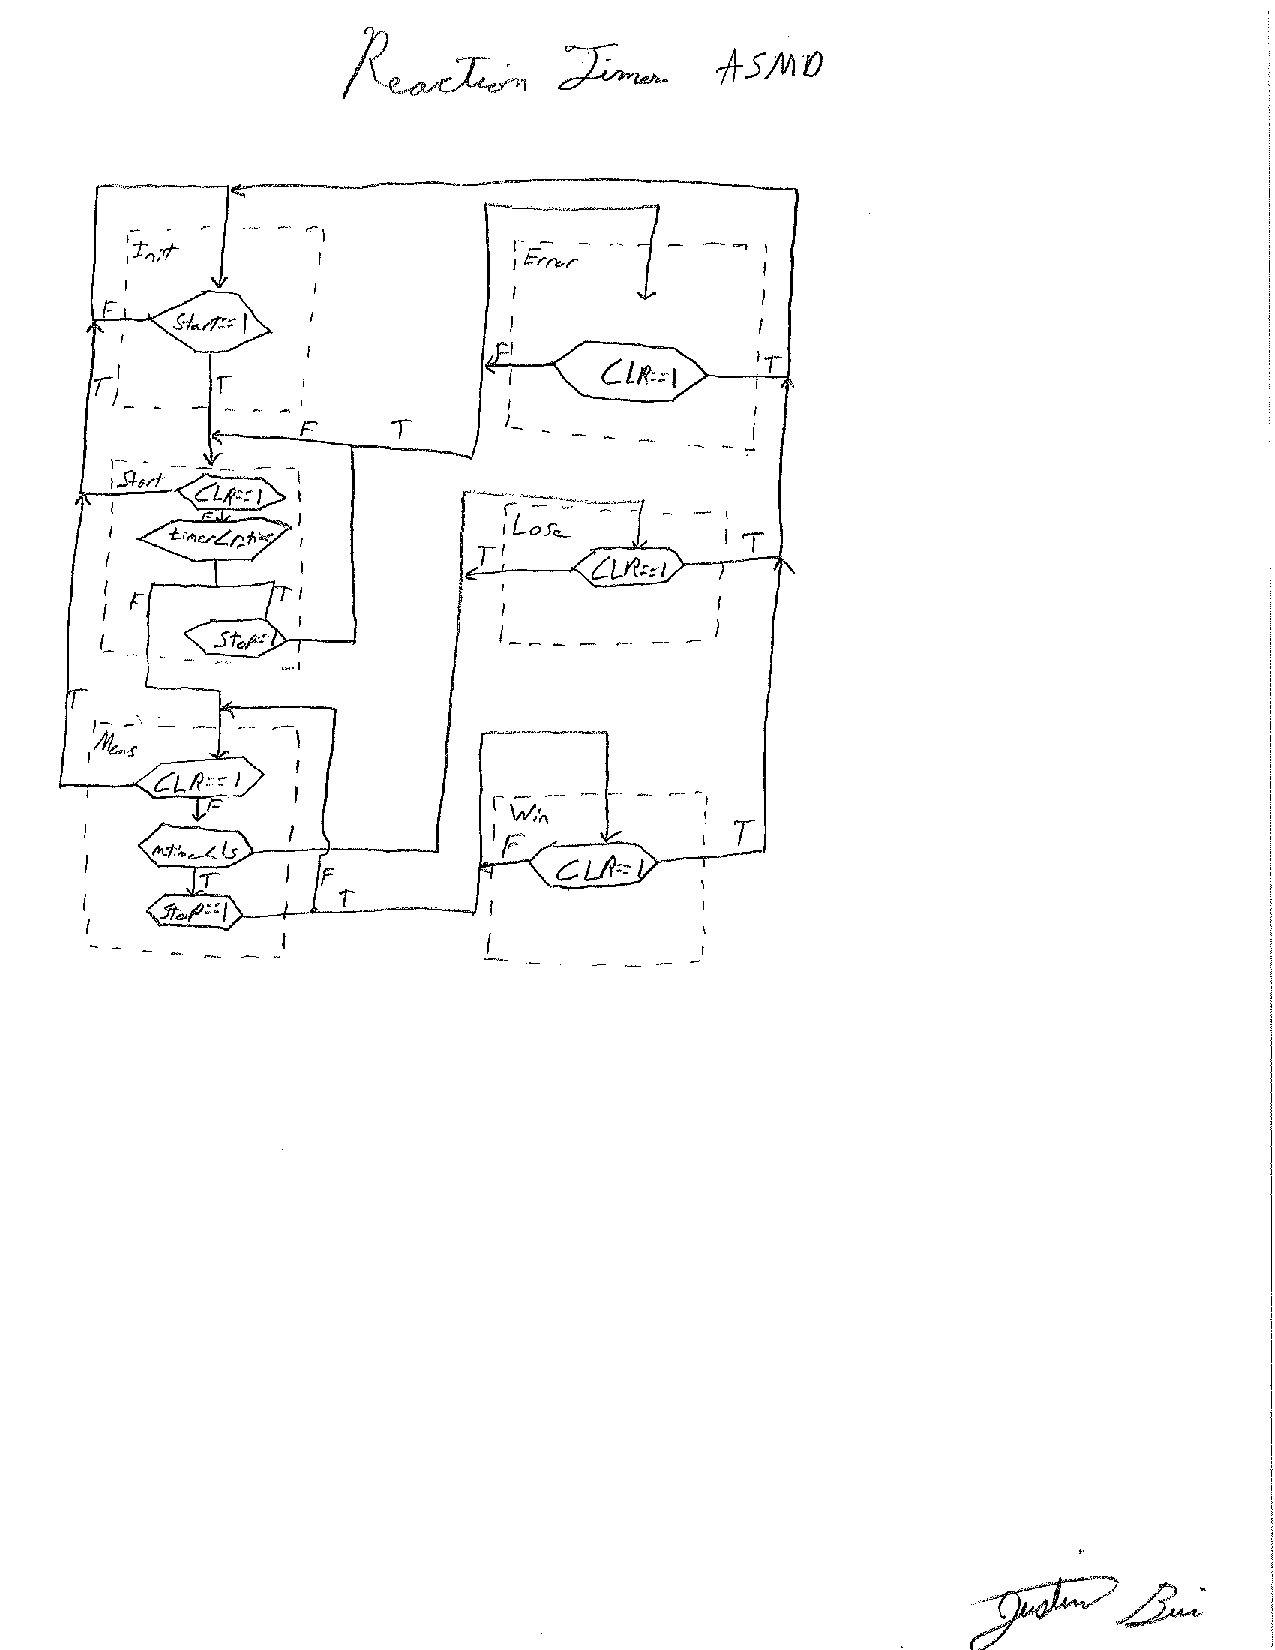
\includegraphics[width=.9\linewidth]{pdfs/reaction_timer_asmd.pdf}
	\caption{Initial ASMD with basic transitions}
	\label{fig:ASMD1}
\end{figure}

\begin{figure}
	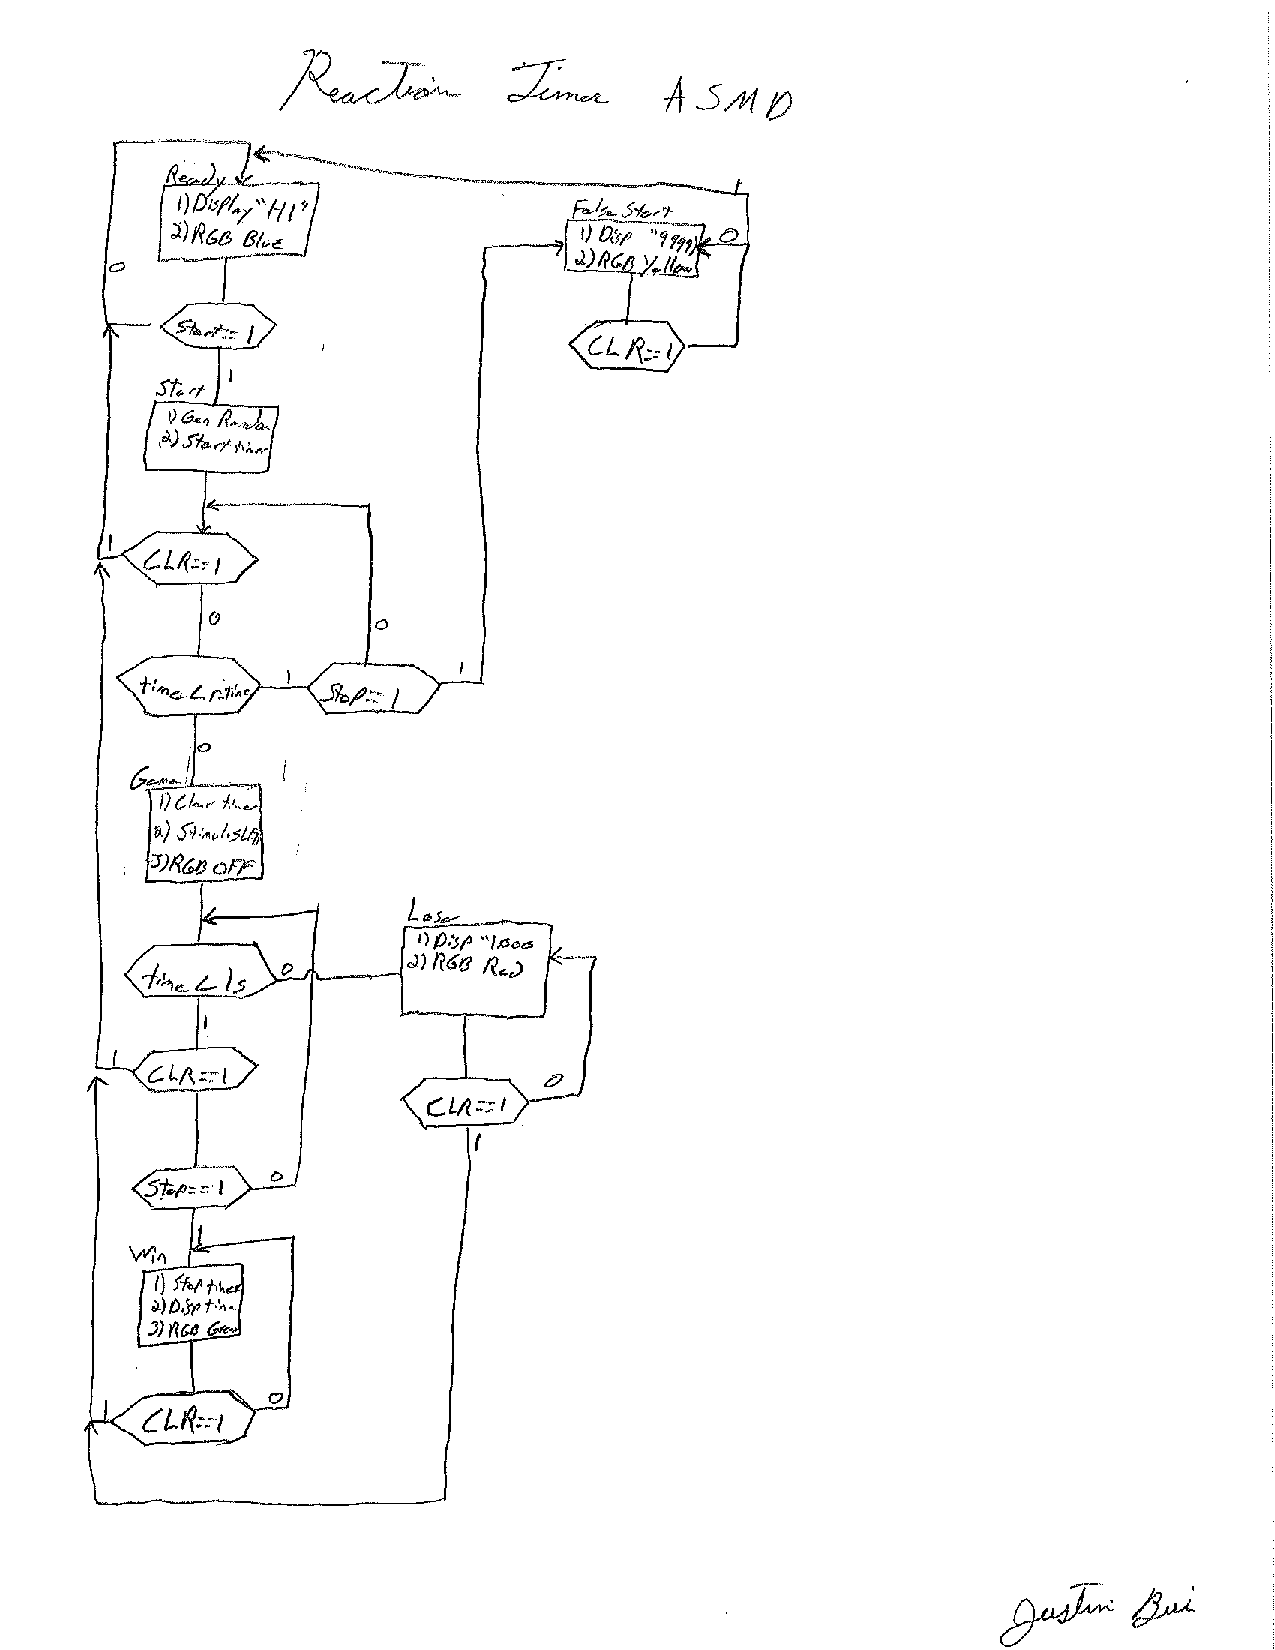
\includegraphics[width=.9\linewidth]{pdfs/reaction_timer_asmd_v2.pdf}
	\caption{Second Draft ASMD with More Detail}
	\label{fig:ASMD2}
\end{figure}

As you can see, I have emphasized simplicity and code reusability for this project. In the next section, I will go in to more detail regarding the functionality of the Reaction Timer.

\newpage

\section{Reaction Timer Functionality}
As previously mentioned, the Reaction Timer makes use of a number of different elements, including the stopwatch and display modules. I have designed the stopwatch module to emulate the stopwatches used by coaches for athletic events. I've designed the stopwatch to work as a Binary Coded Decimal timer, counting up to 9 and incrementing the next decade. I have set each digit to be a 4 bit number (as seen in the code snipit below. This allows for 0-9 on the ms digits, and 0-F for the seconds digit. I have not capped the seconds digit at 9 to allow for the random 2-15 second time interval to make use of that value (maximizing code reusability).

\begin{lstlisting}
    //Declarations
    localparam DVSR = 100000;
    //milisecond registers
    logic [24:0] ms_reg;
    logic [24:0] ms_next;
    
    //decade registers (seconds, ds, cs, ms)
    logic [3:0] d3_reg, d2_reg, d1_reg, d0_reg;
    logic [3:0] d3_next, d2_next, d1_next, d0_next;
\end{lstlisting}

For the 7-Segment display control, I have modified the values for Hex codes A and B (1010 and 1011) to display H and I. The code segment below shows the case statement used to "decode" the number to the required display settings.

\begin{lstlisting}
always_comb
begin
        case(val)
             4'h0: sseg[6:0]=7'b1000000; // '0'
             4'h1: sseg[6:0]=7'b1111001; // '1'
             4'h2: sseg[6:0]=7'b0100100; // '2'
             4'h3: sseg[6:0]=7'b0110000; // '3'
             4'h4: sseg[6:0]=7'b0011001; // '4'
             4'h5: sseg[6:0]=7'b0010010; // '5'
             4'h6: sseg[6:0]=7'b0000010; // '6'
             4'h7: sseg[6:0]=7'b1111000; // '7'
             4'h8: sseg[6:0]=7'b0000000; // '8'
             4'h9: sseg[6:0]=7'b0010000; // '9'
             4'ha: sseg[6:0]=7'b0001001; // 'H'
             4'hb: sseg[6:0]=7'b1001111; // 'I' 
             4'hc: sseg[6:0]=7'b0000110; // 'E' 
             4'hd: sseg[6:0]=7'b0000110; // 'E' 
             4'he: sseg[6:0]=7'b0000110; // 'E' 
             default: sseg[6:0]=7'b1111111; 
         endcase
         sseg[7] = dp;
 end
\end{lstlisting}

The final submodule used for the implementation of the Reaction Timer is the random number generator. I made use of Dr. Schubert's 168 bit Fibonacci Pi generator, modified to grab 4 arbitrary bits (in this case 110-113 of the machine state]. The random number generator is constantly running, making it more difficult to predict the timing.


\smallskip
To address the issue of the constantly running random number generator, I've made use of an additional register which stores the random number (in seconds). This prevents the random time from changing while the game is in the Start state.


\smallskip
The top level design, in addition to implementing the modules mentioned above, defines the remaining game logic. This logic covers the state transitions, display configurations (LEDs and 7-Segment Display values), memory registers (timer values, state values, etc, seen below).  Since much of this code is heavily commented and exceeds the marigins for this document, I have posted the code on GitHub to be viewed at anytime. it may be found at: The complete code can be found on github.

\newpage
\section{Design Verification}
The Reaction Timer has been verified through operation and manual testing. By taking advantage of the RGB LED, I am able to determine which state the device is in, as well as verify the timing with an external source. You can see in Table \ref{table:table1} that the RGB LED color indicates which state it is currently in. For future designs, I plan on taking advantage of the simulation techniques to quickly verify the design. Since this design was manually verified, I have provided video documentation showing the functionality of the system. To support the video, below you can see images of the game in it's various states.

\begin{center}
	\begin{figure}
		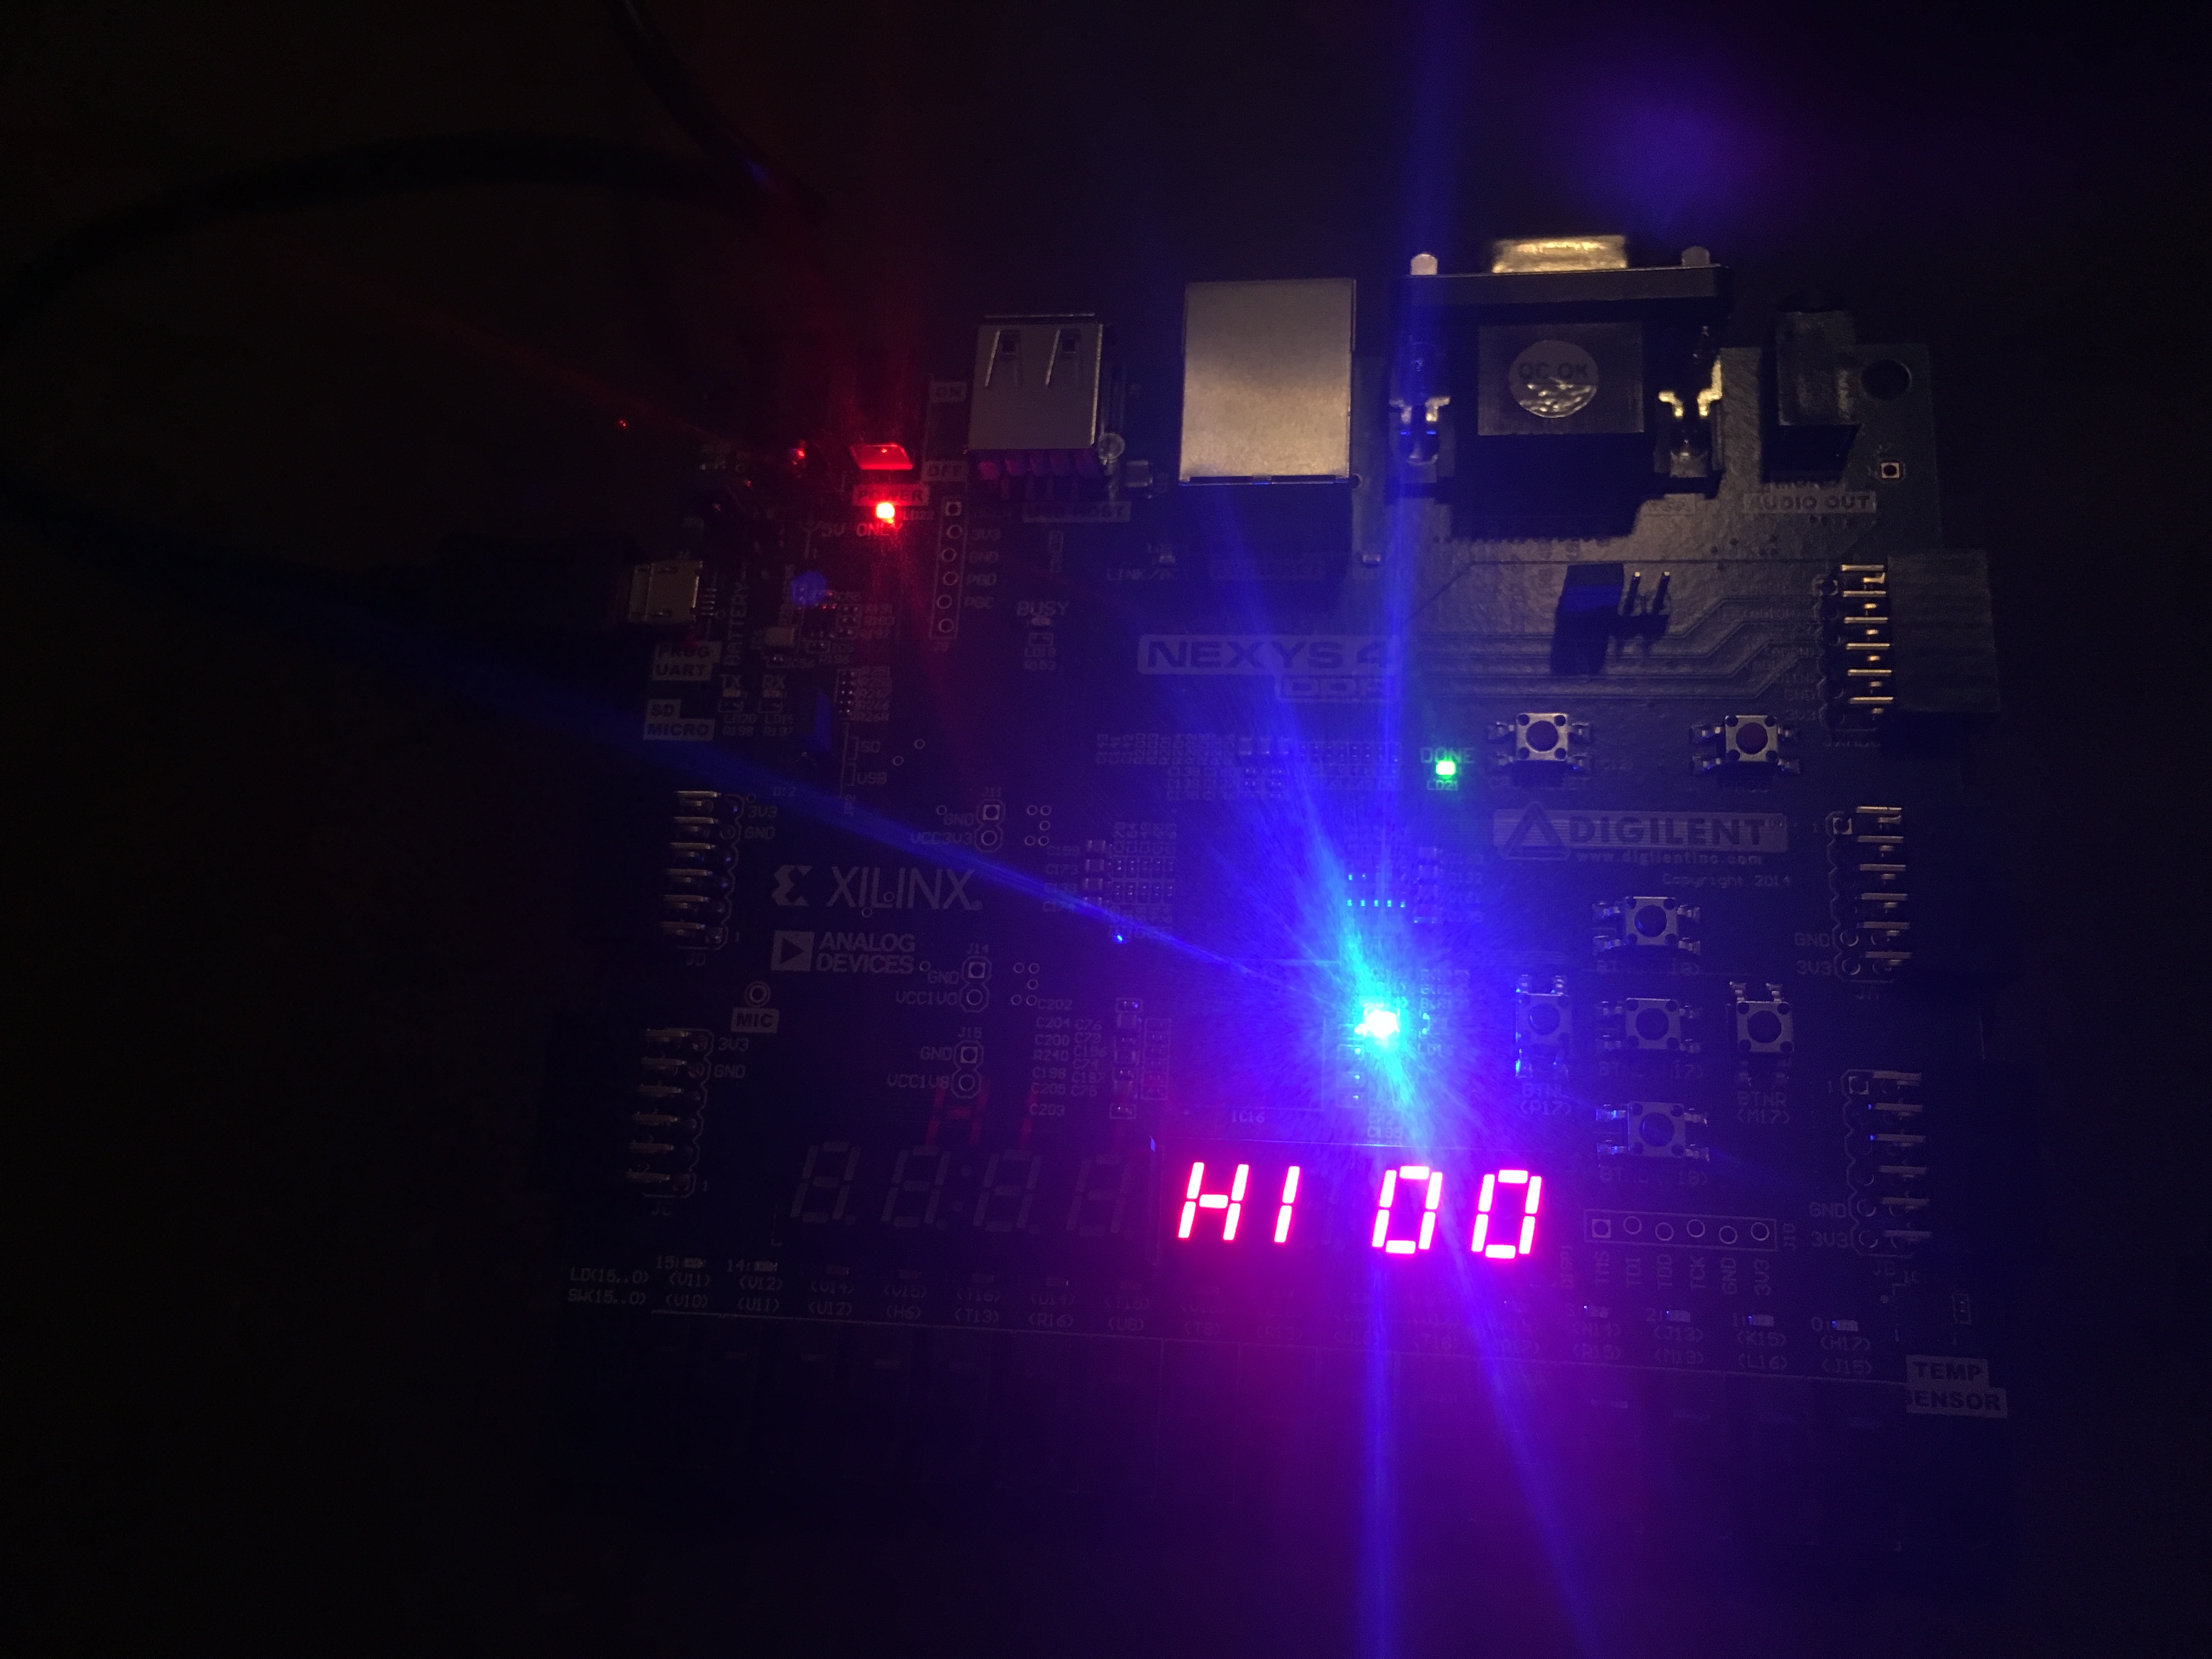
\includegraphics[width=.9\linewidth]{Ready.JPG}
		\caption{Ready State: Blue RGB LED and HI message}
		\label{fig:ReadyImg}
	\end{figure}

	\begin{figure}
		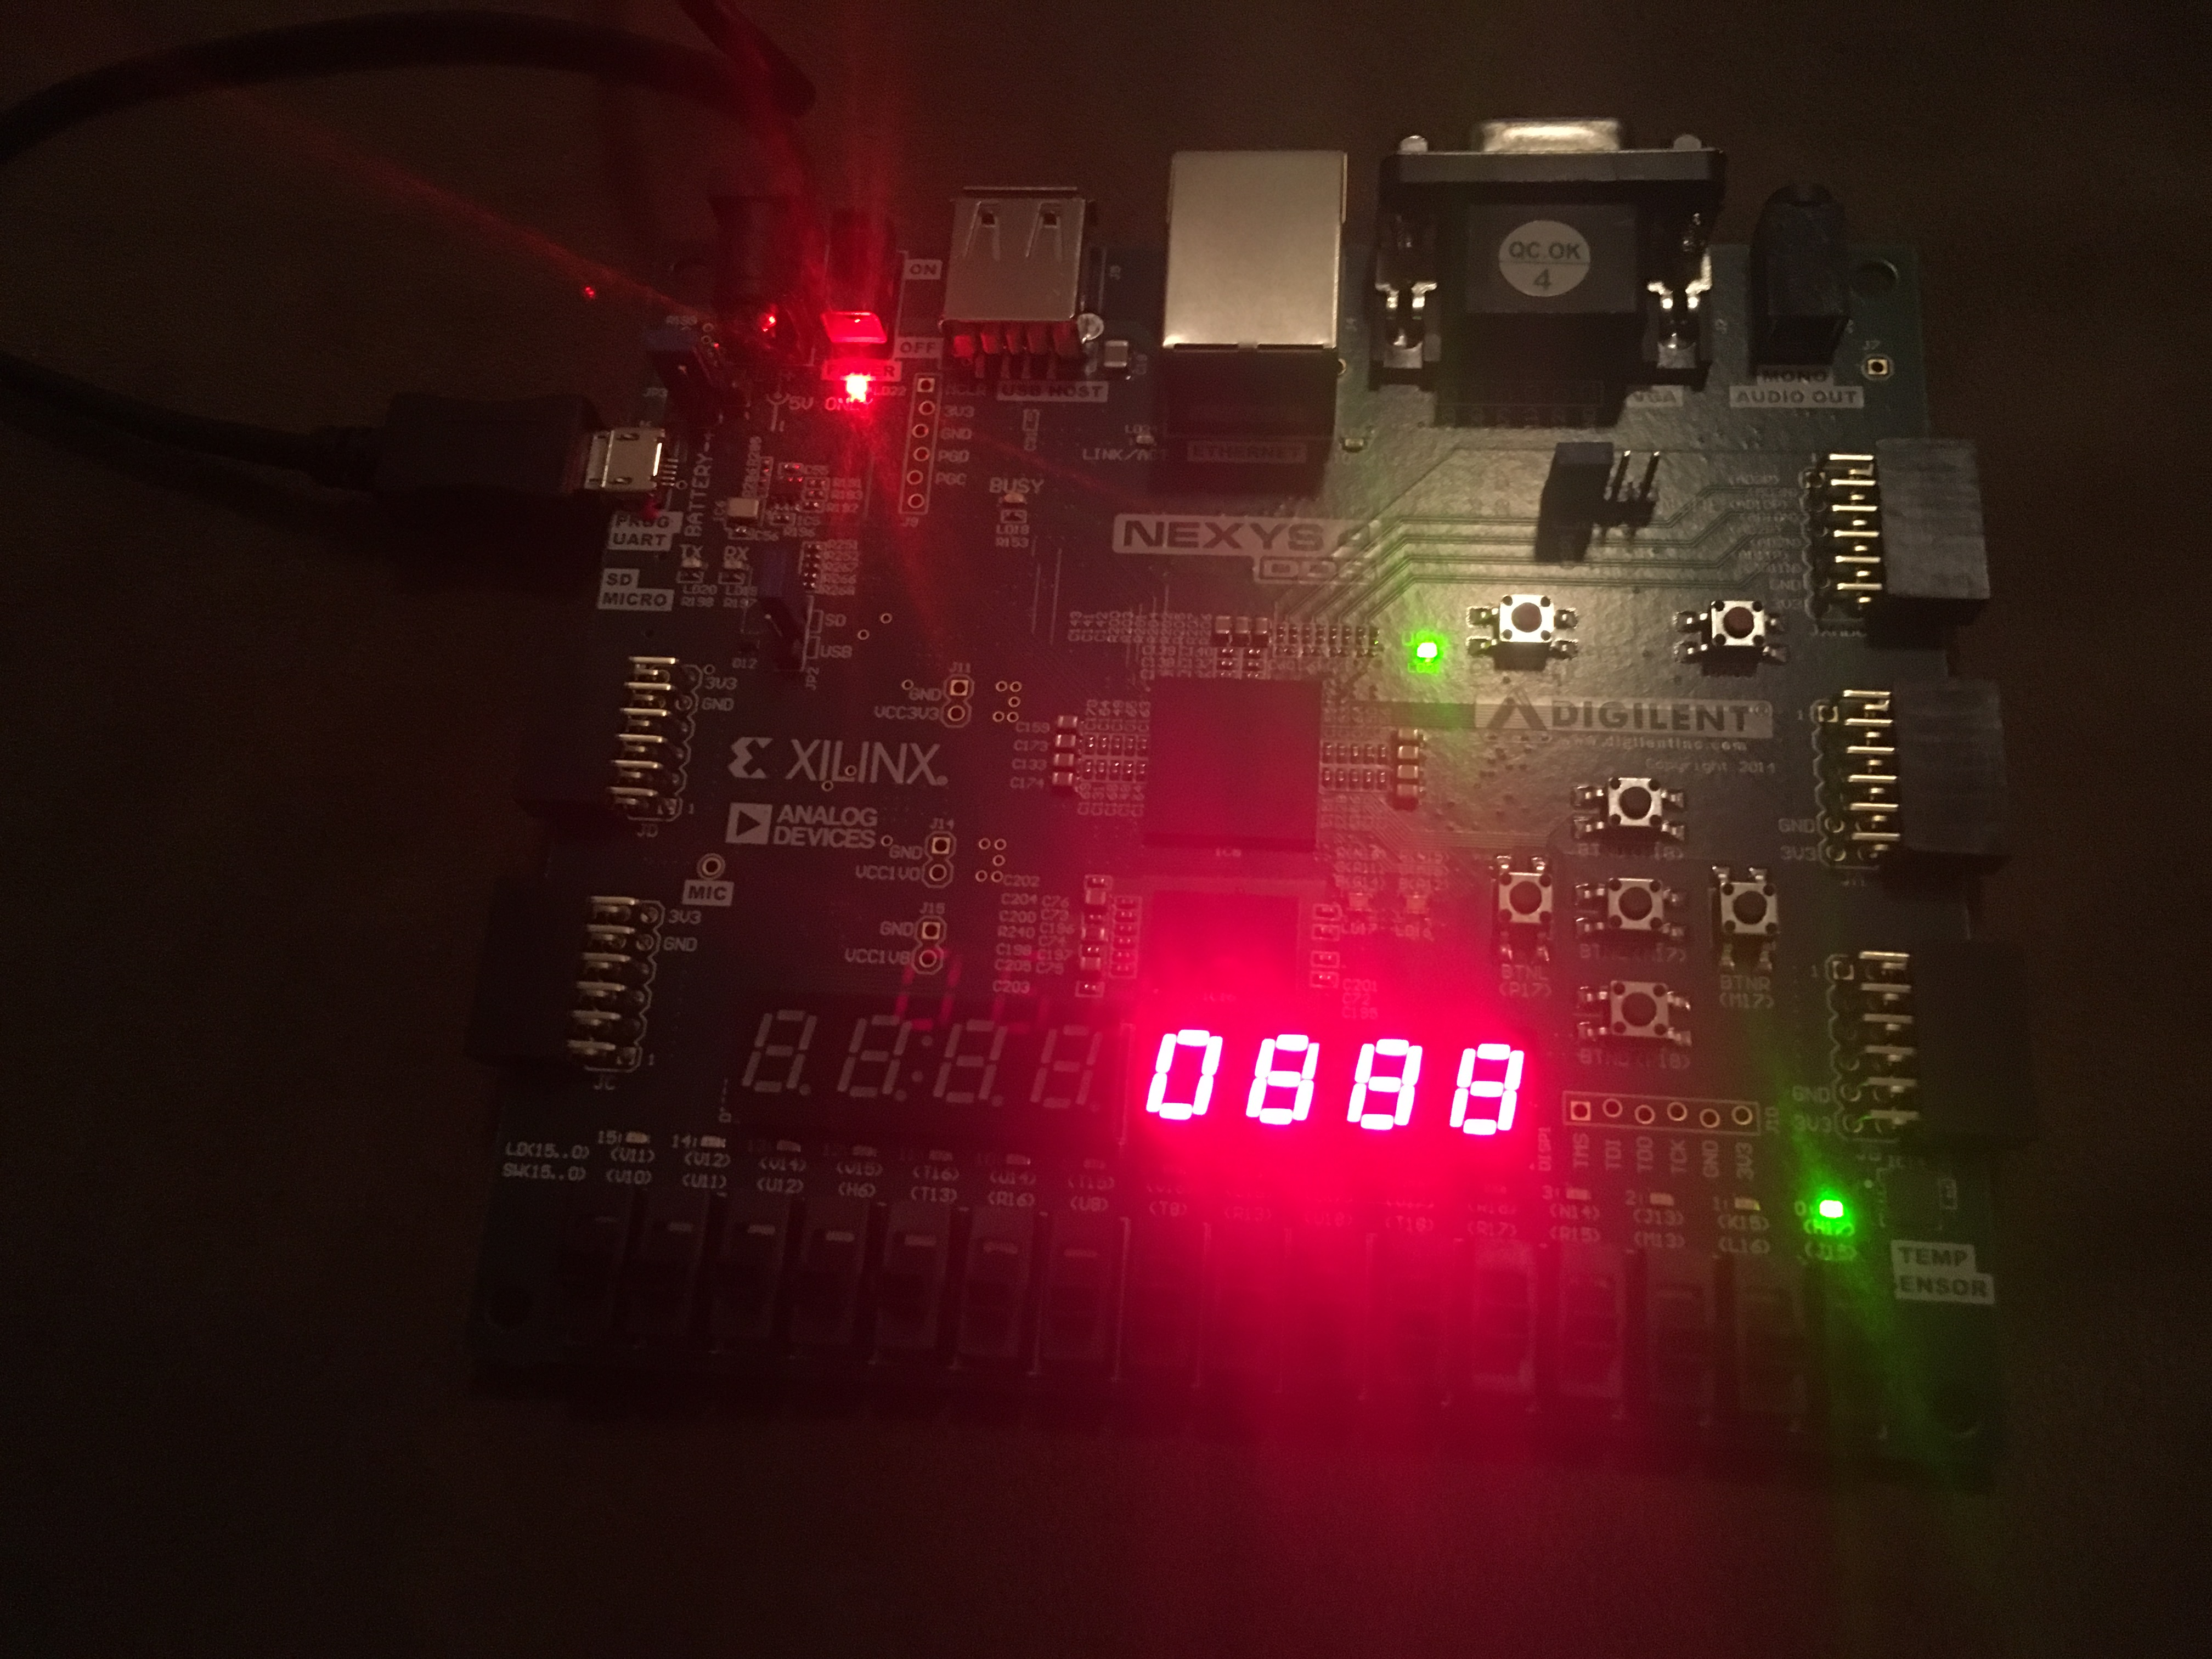
\includegraphics[width=.9\linewidth]{Game.JPG}
		\caption{Game State: Stimulus LED, No RGB LED, and Current Time}
		\label{fig:GameImg}
	\end{figure}

	\begin{figure}
		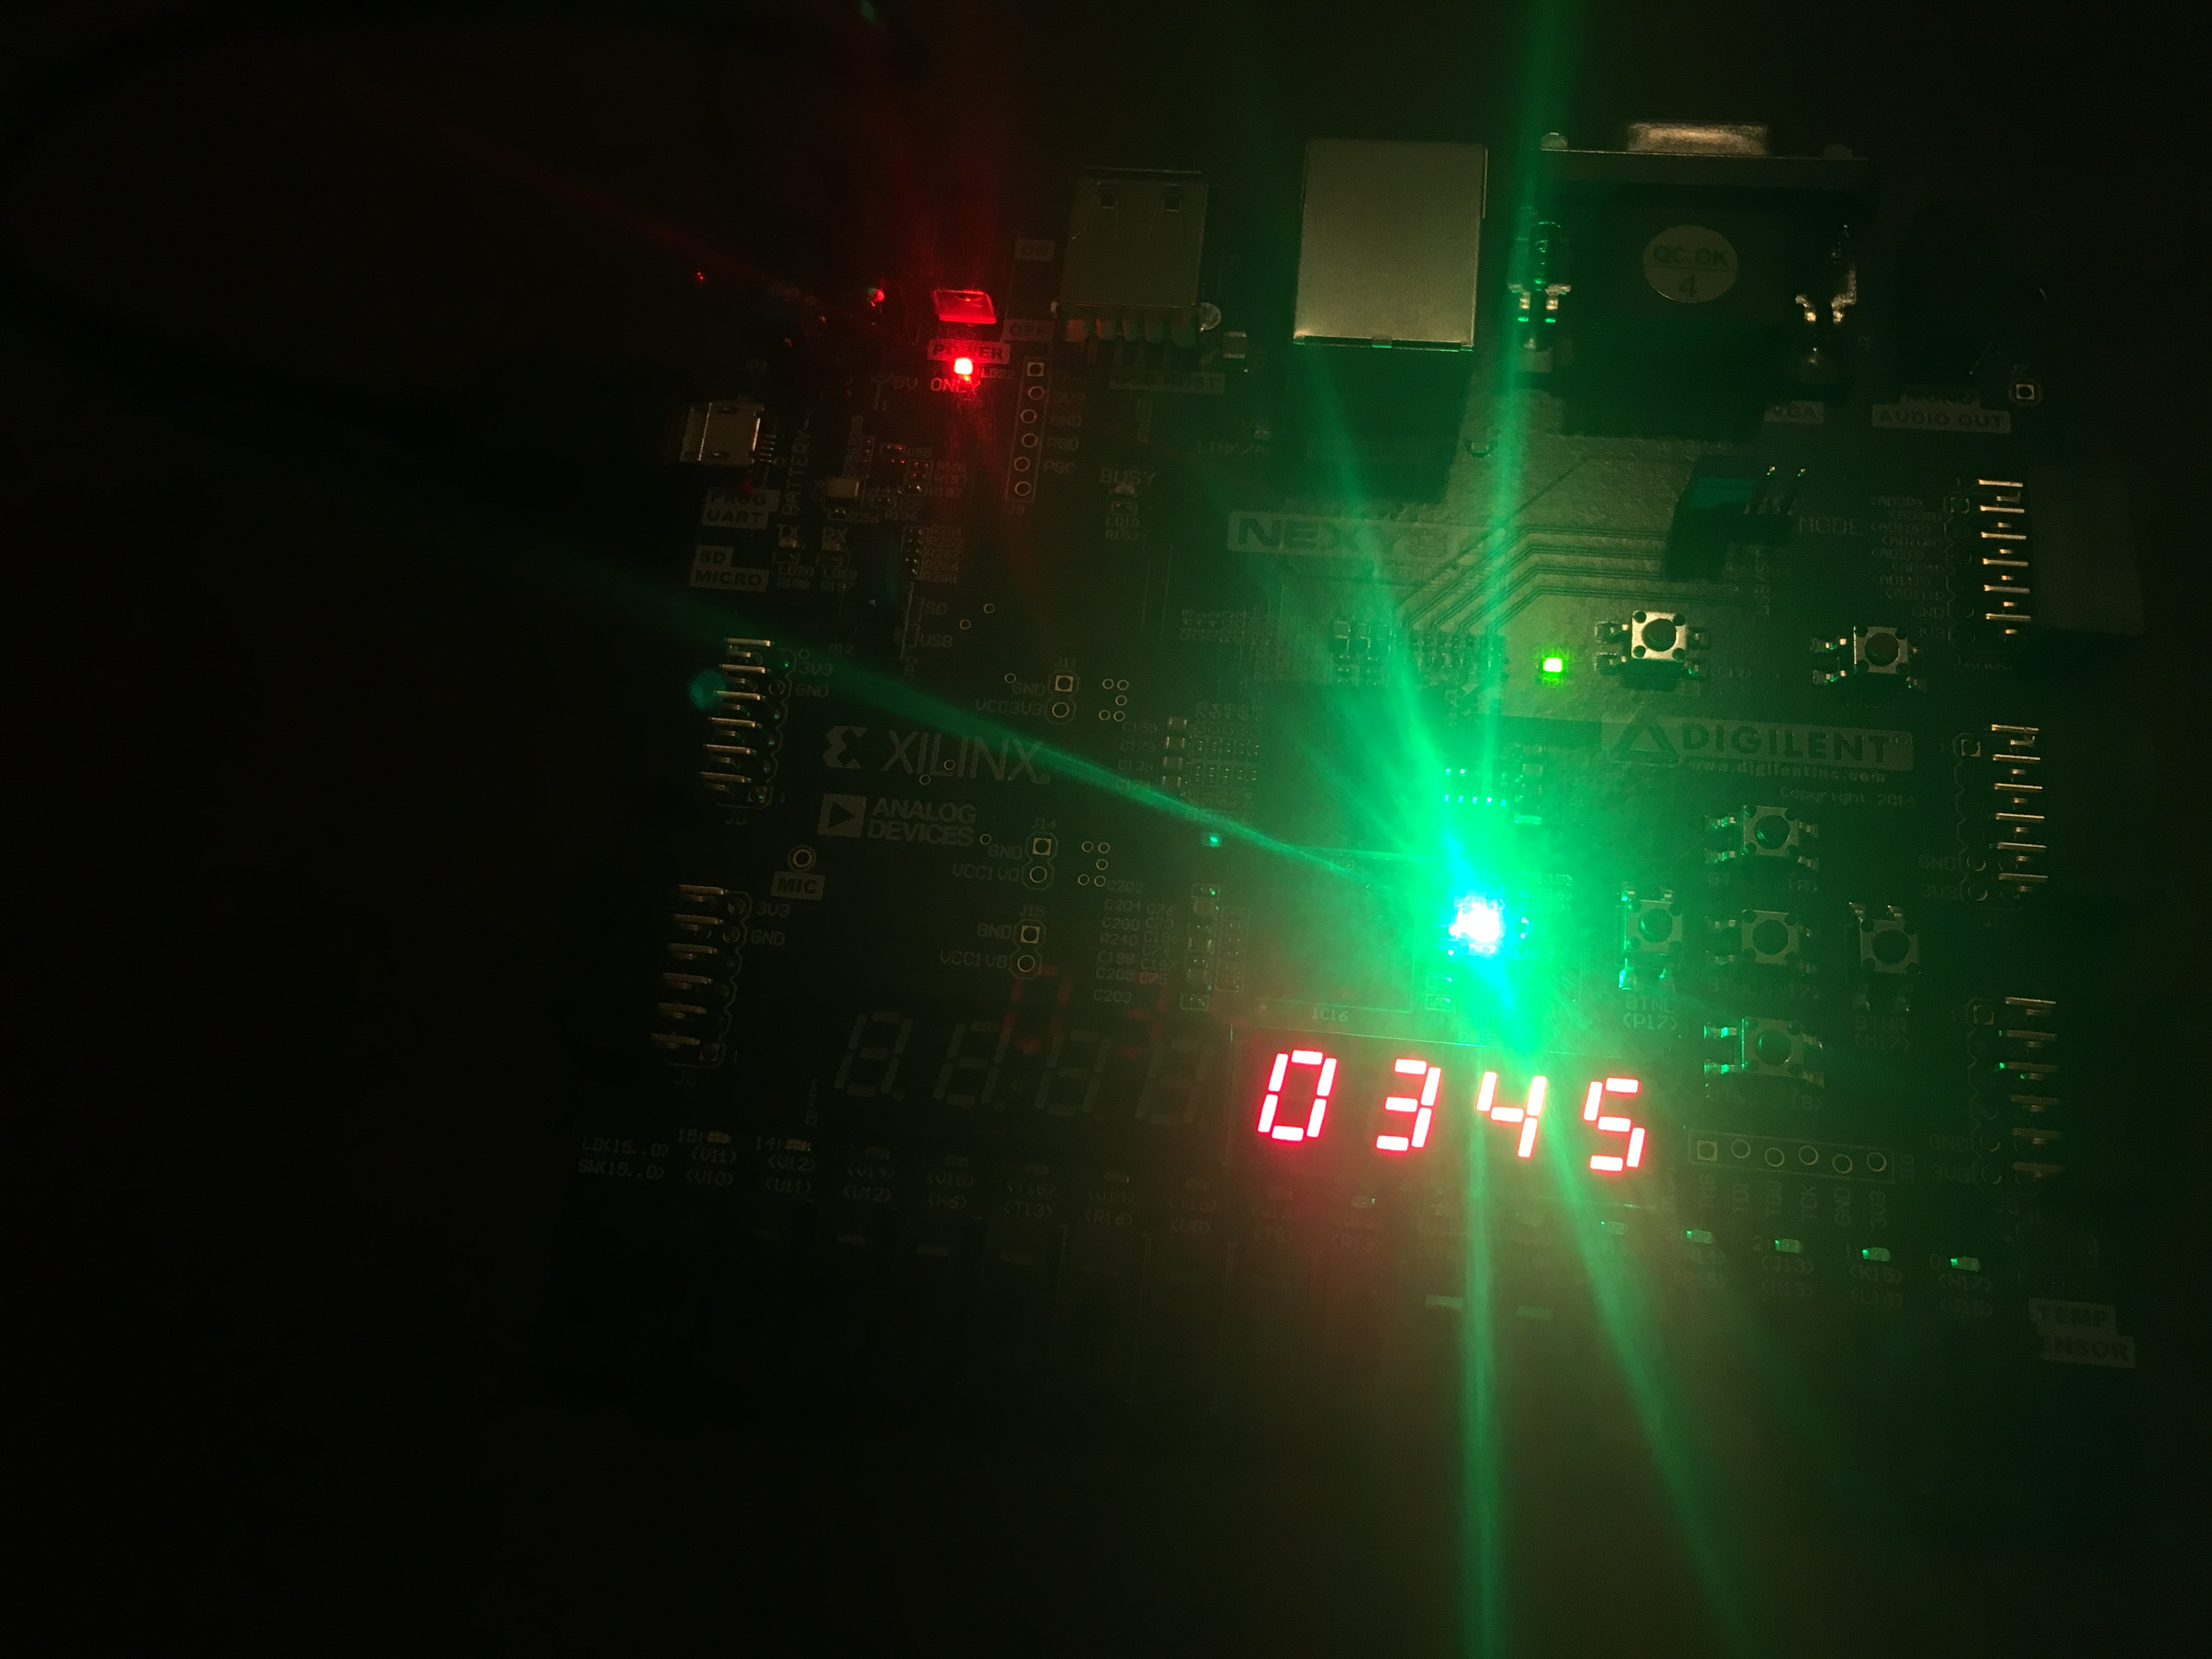
\includegraphics[width=.9\linewidth]{Win.JPG}
		\caption{Win State: Green RGB LED and Reaction Time}
		\label{fig:WinImg}
	\end{figure}

	\begin{figure}
		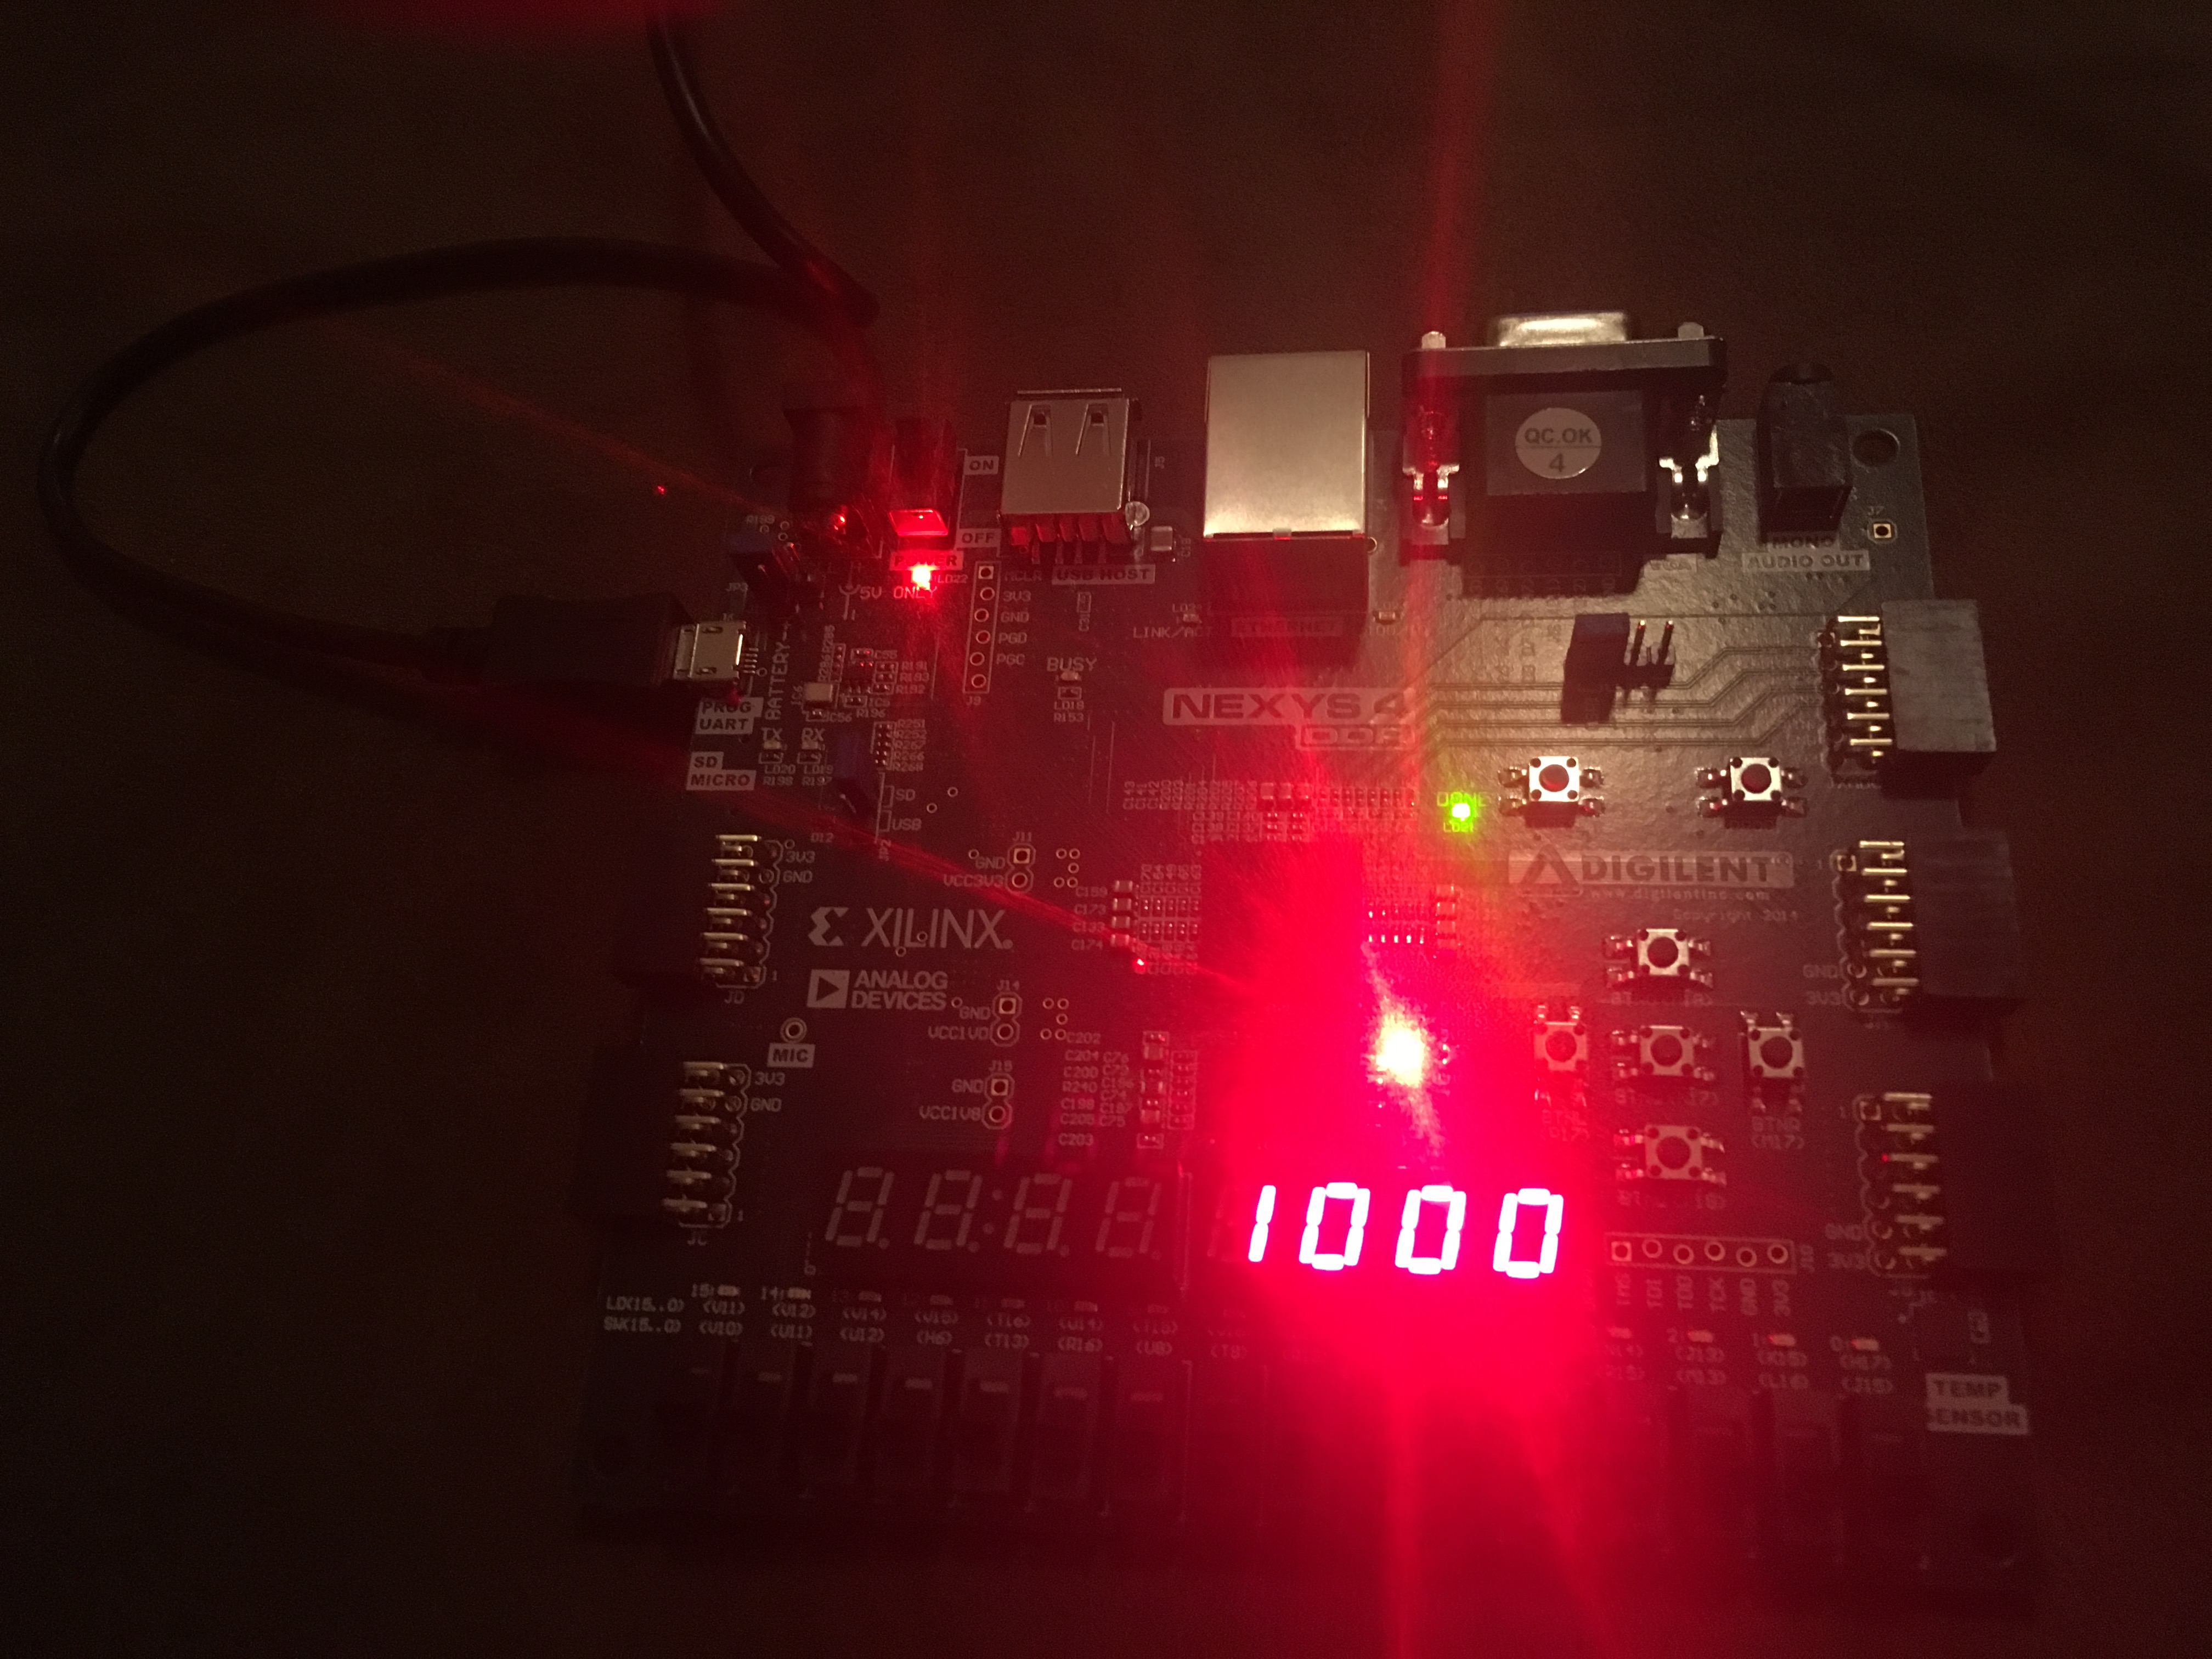
\includegraphics[width=.9\linewidth]{Lose.JPG}
		\caption{Lose State:  Red RGB LED, and 1000 Count}
		\label{fig:LoseImg}
	\end{figure}

	\begin{figure}
		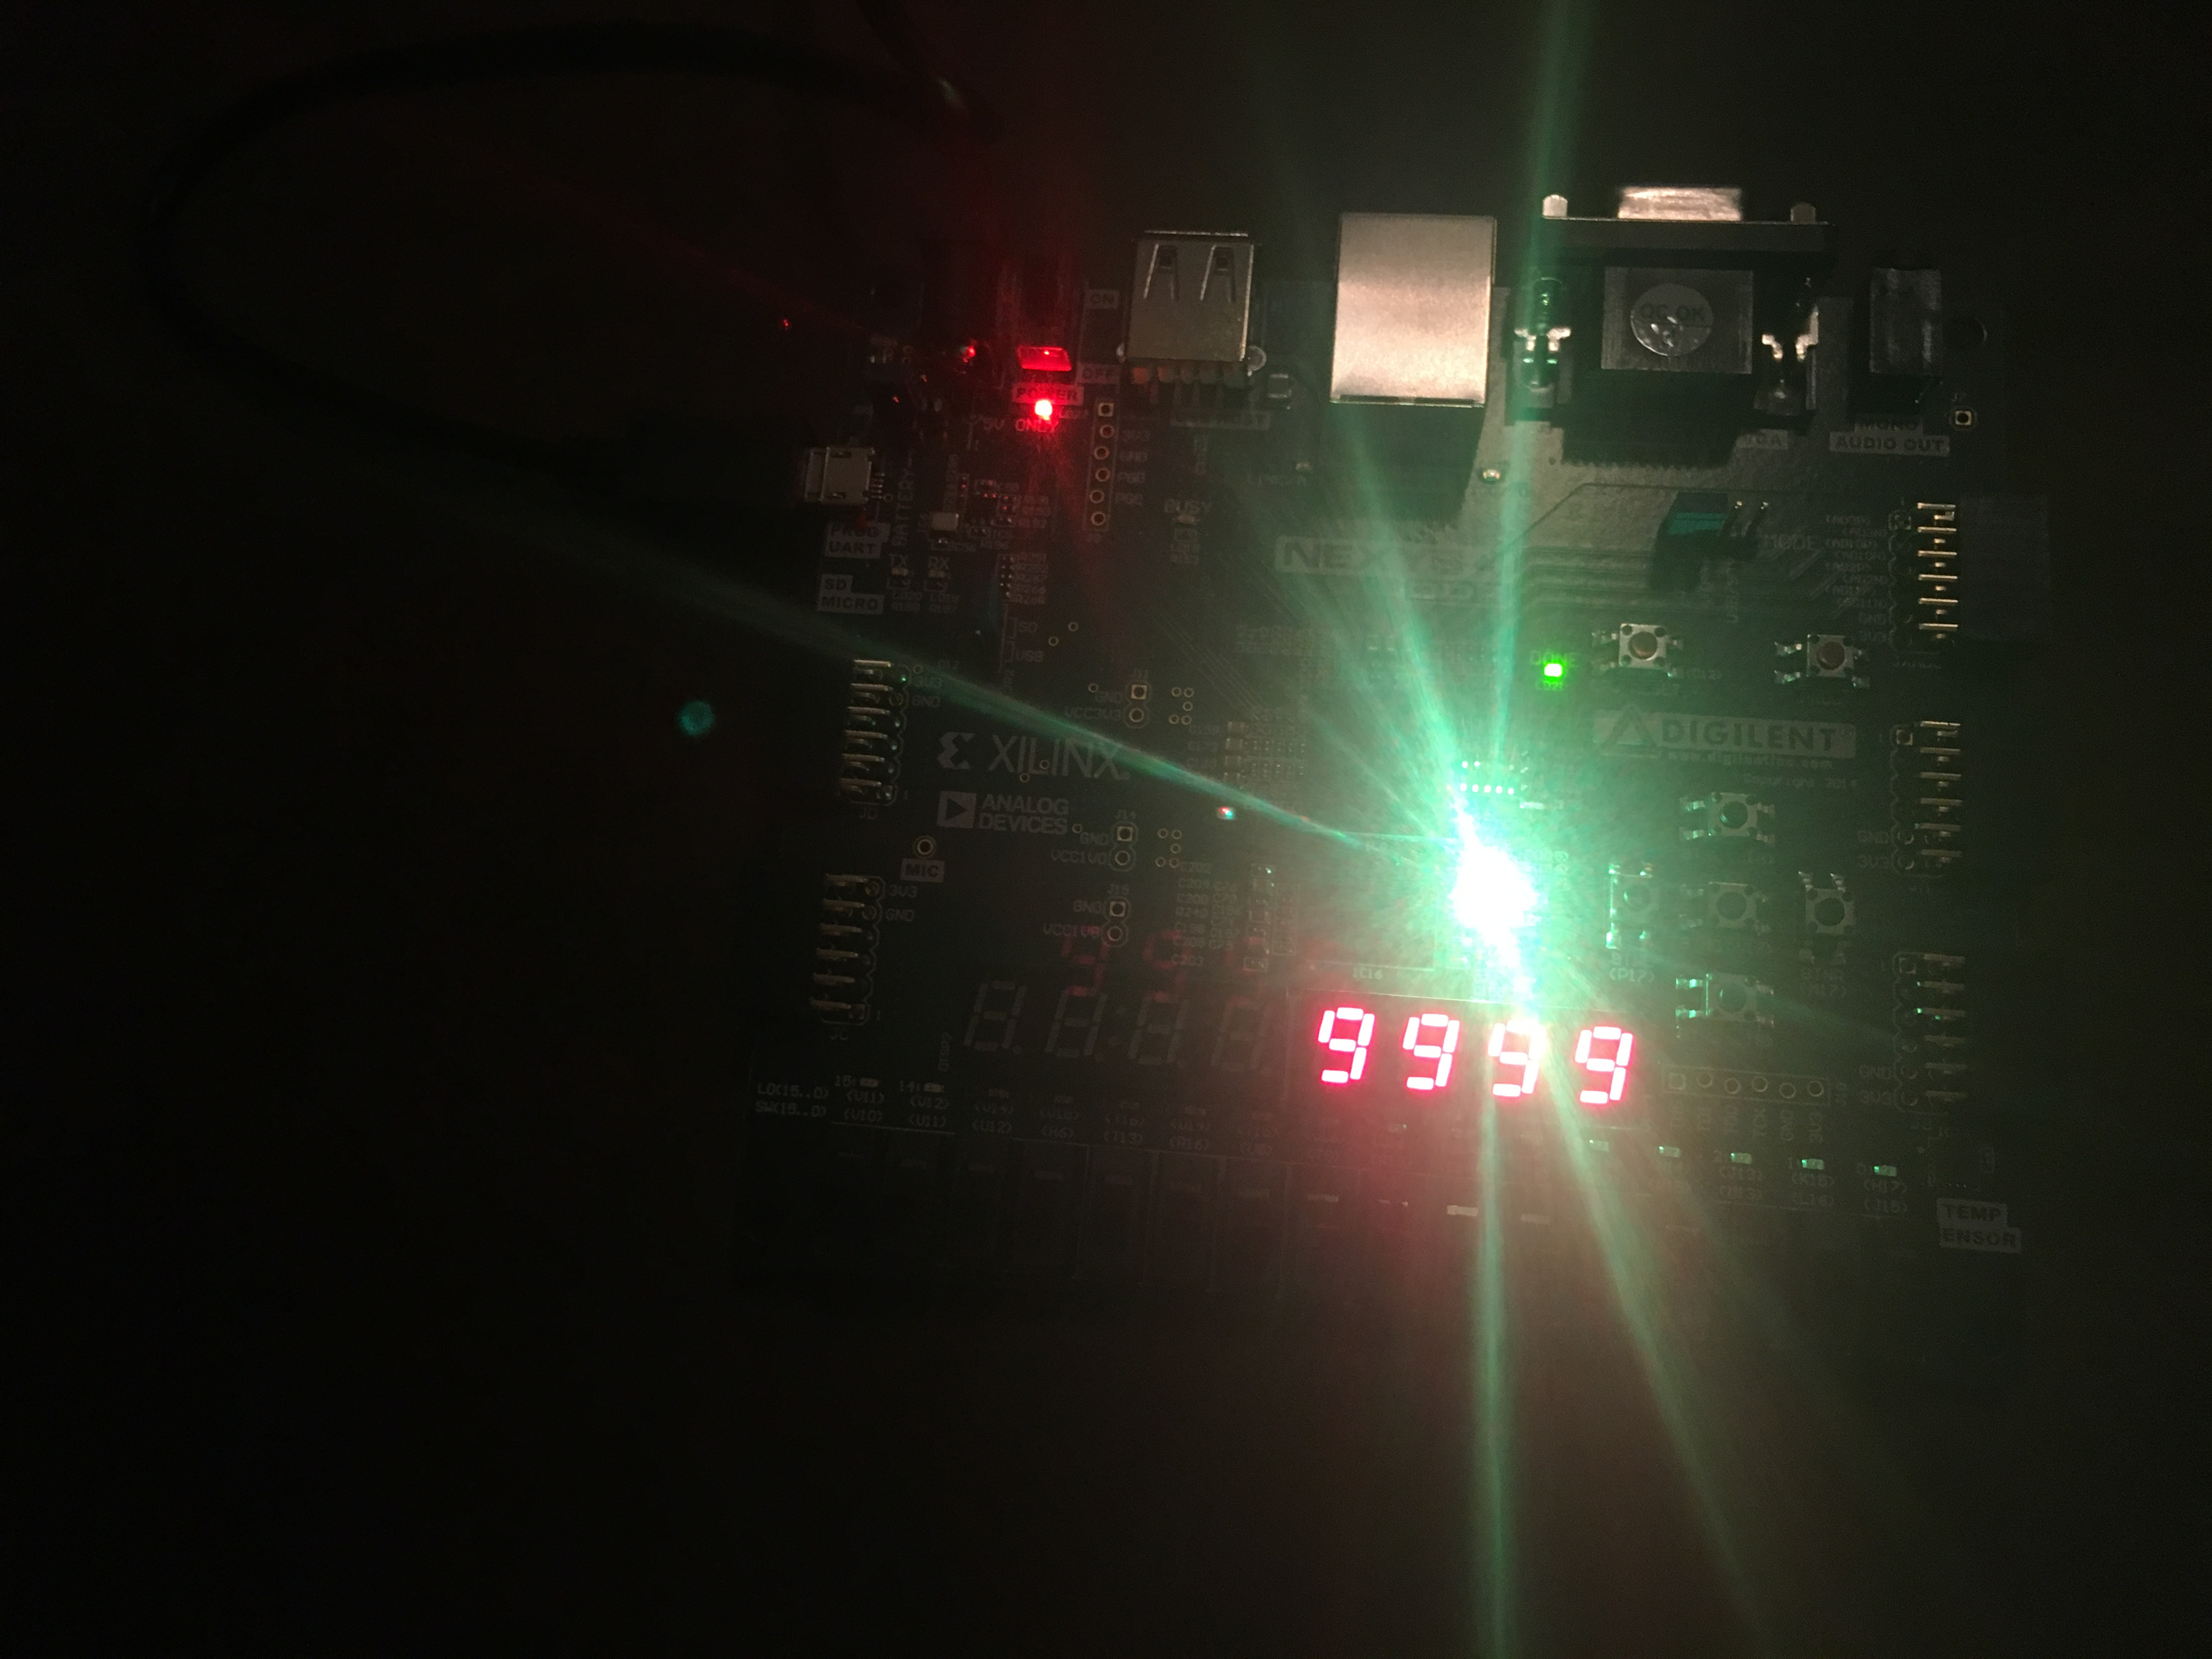
\includegraphics[width=.9\linewidth]{Error.JPG}
		\caption{Error State: Yellow LED and 9999 Display Value}
		\label{fig:ReadyImg}
	\end{figure}
\end{center}


\end{document}